\documentclass[prl,twocolumn]{revtex4-1}

\usepackage{graphicx}
\usepackage{color}
\usepackage{latexsym,amsmath}
\usepackage{amsfonts}
\usepackage{caption}

\definecolor{linkcolor}{rgb}{1.0,0.647,0.0} %hyperlink
\usepackage[pdftex,colorlinks=true, pdfstartview=FitV, linkcolor= linkcolor, citecolor= linkcolor, urlcolor= linkcolor, hyperindex=true,hyperfigures=true]{hyperref} %hyperlink%

\usepackage{enumitem}
\setlist[itemize]{leftmargin=*}


\setcounter{secnumdepth}{2}

\renewcommand{\thesection}{\arabic{section}}
\renewcommand{\theequation}{\thesection.\arabic{equation}}

\makeatletter
\@addtoreset{equation}{section} % Reset equation counter at each section
\makeatother

\begin{document}

\title{Quantum Optics and Laser, Lab3 - Gaussian beams and diffraction}



\author{Calandra Buonaura Lorenzo}

\date{\today}


\begin{abstract}

In this experiment, we investigate the wave-like properties of light by studying the behavior of Gaussian beams as they propagate through optical systems. Our goal is to explore how lenses shape the spatial characteristics of these beams and to analyze diffraction patterns that arise when light encounters obstacles. By employing carefully designed lens setups, we measure the beam waist, divergence, and focusing properties, verifying the theoretical predictions of Gaussian optics. Additionally, we examine diffraction phenomena to illustrate the interplay between beam coherence and wavefront curvature.

\end{abstract}

\maketitle

\section{Introduction}

Laser beams are widely used in numerous scientific and industrial applications due to their high coherence, monochromaticity, and directional properties. Among the different laser beam models, Gaussian beams represent an idealized yet practical framework for describing light propagation, including intensity distribution, divergence, and interactions with optical components. 

The primary aim of this experiment is to investigate the fundamental properties of Gaussian beams and their interactions with optical elements such as lenses and splits. Specifically, the experiment seeks to analyze the transverse intensity distribution, the effects of beam propagation through a lens, and the diffraction phenomena resulting from interaction with a circular aperture.


\section{Theoretical framework}

Gaussian beams represent an idealized model of laser light propagation, characterized by their unique spatial distribution and predictable behavior under linear optical transformations. These characteristics make Gaussian beams perfect for building an analytical model of light, which is described in the following.

\subsection{Intensity distribution}

The intensity of a Gaussian beam, $I(r)$, is a function of the radial distance $\rho = \sqrt{x^2 + y^2}$ from the beam's central axis and the propagation distance $z$. It is given by:
\begin{equation}
I(\rho, z) = I_0 \left( \frac{W_0}{W(z)} \right)^2 \exp\left(-2 \frac{\rho^2}{(W(z))^2}\right),
\end{equation}
where $I_0$ is the peak intensity at the beam waist ($z = 0$). At any value of $z$, the intensity is a Gaussian function of the radial distance $\rho$ (hence the name Gaussian beam); the factor $\left(W_0 / W(z)\right)^2$ accounts for the spreading of the beam as it propagates, while the exponential term describes the radial decay of the intensity~\cite{pap1}.

\subsection{Optical power}

The total optical power carried by the beam is the integral of the optical intensity over any transverse plane (at fixed position $z$):
\begin{equation}
P = \int_{0}^{\infty} I(\rho, z) \, 2\pi \rho \, \mathrm{d}\rho.
\end{equation}
which yields:
\begin{equation}
    P = \frac{1}{2} I_0 (\pi W_0^2)
\end{equation}

\subsection{Gaussian beam width}
\label{sec:gaussian_beam_width}
Fixed $z$, the beam intensity assumes its peak value on the beam axis and it's decreased by the factor $1/e^2$ at the radial distance $\rho = W(z)$; this distance is called \textit{beam radius} (or \textit{beam width})~\cite{pap1}. For a Gaussian beam, this quantity corresponds to $2\sigma$ and it's important as 86\% of the total power is carried within a circle of radius $W(z)$. Moreover, this quantity varies with the propagation distance $z$ and the dependency is described by:
\begin{equation}
\label{eq:beam_radius}
W(z) = W_0 \sqrt{1 + \left(\frac{z}{z_R}\right)^2},
\end{equation}
where $W_0$ is the beam waist, representing the minimum radius of the beam (when $z=0$), and $z_R$ is the Rayleigh range, given by:
\begin{equation}
\label{eq:W_0_and_z_R}
z_R = \frac{\pi W_0^2}{\lambda}.
\end{equation}
where $\lambda$ is the wavelength of the laser. The Rayleigh range defines the distance from the beam waist at which the beam area doubles, marking the transition between the near-field and far-field regimes.

\subsection{Effect of lenses}
When a Gaussian beam passes through a lens, its width undergoes a transformation determined by the lens' focal length $f$ and the beam's initial parameters. This time, the evolution of the beam width $W(z)$ along the propagation axis $z$ is given by:

\begin{equation}
\label{eq:beam_radius_lens}
W(z) = W_0 \sqrt{1 + \left( \frac{z - f}{z_R} \right)^2},
\end{equation}

where $W_0$ and $z_R$ are defined as before~\cite{pap1}. As we can see, the total effect of the lens is to modify the Gaussian beam by introducing a new beam waist with altered width and position, effectively changing its divergence and focus characteristics.

\subsection{Diffraction}
\label{sec:diffraction_theory}

As Gaussian beams encounter apertures or obstacles, they exhibit the typical effects of waves; in particular, we focus on diffraction effects, which are characterized by the Fresnel number, a dimensionless parameter that governs the beam's propagation regime~\cite{pap2}. The Fresnel number is defined as:

\begin{equation}
\label{eq:fresnel_number}
N_F = \frac{a^2}{\lambda z},
\end{equation}

where $a$ is the radius of the aperture or obstacle, $\lambda$ is the wavelength of the beam and $z$ is the distance from the aperture to the observation plane.

The Fresnel number distinguishes between diffraction regimes:
\begin{itemize}
    \item For $N_F \gg 1$, the beam propagation is in the near-field or Fresnel regime, where diffraction patterns are complex and depend on the exact aperture geometry.
    \item For $N_F \ll 1$, the beam reaches the far-field or Fraunhofer regime, where the diffraction pattern simplifies and the beam spreads with a Gaussian intensity profile.
\end{itemize}

We are interested in the case of circular diffraction: in this case the diffraction figure will be described by alternating concentric bright and dark rings. The number of bright or dark fringes observed corresponds approximately to the Fresnel number~\cite{pap2}:
\begin{equation}
\text{\# of fringes} \approx \lfloor N_F \rfloor.
\end{equation}
This relationship arises because each Fresnel zone contributes a phase difference to the interference, and the total number of zones is related to $N_F$.

\section{Apparatus}

The experimental setup used in this work involves several components, each playing a critical role in the measurement and manipulation of the laser beam, complete by a CCD camera for data collection. Below is a detailed description of all the elements of the apparatus used in the experiment:

\begin{enumerate}
    \item \textbf{Gas tube laser:} The laser used in this experiment is a gas tube laser that emits coherent light with a wavelength of $\lambda = 633 \, \text{nm}$. This laser provides a stable, monochromatic light source, which ensures that the diffraction patterns observed on the CCD camera are due to well-defined wavefronts, necessary for analyzing the diffraction effects accurately.
    
    \item \textbf{Polarizer:} A polarizer is used to adjust the polarization of the laser beam before it interacts with other optical components or passes through an aperture.
    
    \item \textbf{CCD camera:} The CCD camera is employed to sense the beam as it impinges on the camera surface. The resolution of the camera is important for capturing fine details in the diffraction pattern: Each pixel of the camera corresponds to a size of 3.45 $\mu m$, allowing for high-resolution imaging of the diffraction fringes.
    
    \item \textbf{Attenuators:} Attenuators are used to reduce the intensity of the laser beam; this is necessary for controlling the brightness of the beam and ensuring that the beam signal is not saturated on the CCD camera.
    
    \item \textbf{Lens:} A lens is used to focus or collimate the laser beam and to observe hoe the Gaussian beam is modified after it. The focal length of the lens determines how the beam spreads after passing through the lens.
    
    \item \textbf{Beam expander:} The beam expander is used to increase the diameter and at the same reduce the divergence of the beam,  ensuring that the diffraction picture propagates uniformly. 
    
    \item \textbf{Small slit:} A small slit is used to allow the laser beam to pass through it, creating diffraction effects that will be recorded on the CCD camera. The size and shape of the aperture are important parameters that affect the diffraction pattern's characteristics, such as fringe spacing and intensity distribution.
    
    \item \textbf{Computer:} A computer is used to display the diffraction pattern collected by the CCD camera.
\end{enumerate}

All components are securely mounted on an optical table, providing a stable and vibration-isolated environment. This setup minimizes external disturbances, such as mechanical vibrations or air currents, which could introduce significant noise into the photon detection process, falsifying the result of the experiment.

\section{Experimental Procedure}

The experiment was conducted in three distinct phases, each designed to study a specific aspect of Gaussian beam behavior and its interaction with optical components:

\begin{figure}[!b]
    \centering
    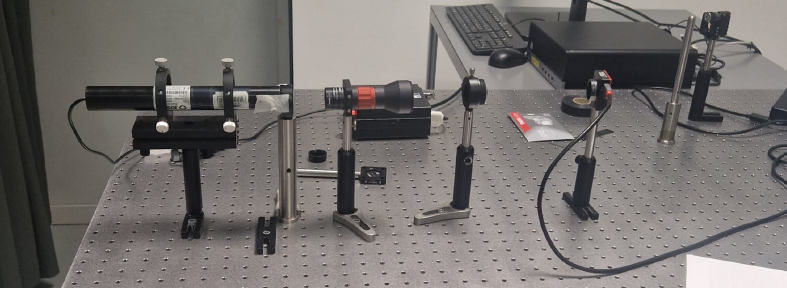
\includegraphics[width=\linewidth]{Images/setup.png}
    \caption{Experimental setup (part 3).}
    \label{fig:setup}
\end{figure}

\begin{enumerate}
  \item \textbf{Study of laser beam behavior:}  
  In the first phase, the laser source emitted a coherent beam of light that directly impinged on the CCD camera. The CCD recorded the transverse intensity distributions of the laser beam, which were displayed on the connected computer in both the $X$ and $Y$ directions. The camera's position was varied along the propagation axis by moving it closer to and farther from the laser source: at each position, the intensity distributions were measured and analyzed to characterize the beam's behavior over different distances.

  \item \textbf{Beam propagation through a lens:}  
  In the second phase, a lens was introduced between the laser source and the CCD camera. The experimental procedure remained similar to the first phase, with the CCD recording the transverse intensity distributions as the camera was moved along the beam's propagation axis. This setup allowed for an investigation of the beam's transformation due to the focusing effect of the lens, including changes in beam width and intensity profile.

  Additionally, the Foucault knife-edge test was used to determine the position of the beam waist after the lens, observing how the Gaussian beam was interrupted at different positions relative to the focus. The observations from this test are as follows:
  \begin{itemize}
    \item \textbf{Before the focus:}  
    When the knife-edge was placed in the beam's path before the focus, the beam was progressively cut starting from one side, which on the CCD camera demonstrated an asymmetric truncation of the beam profile.

    \item \textbf{After the focus:}  
    When the knife-edge was positioned beyond the focus, the beam was cut from the opposite side relative to the pre-focus case, which demonstrated the reversal of the beam's wavefront curvature after the focus.

    \item \textbf{At the Focus:}  
    When the knife-edge was placed precisely at the focal plane, the beam spot on the CCD disappeared suddenly, indicating the location of the beam waist. This abrupt disappearance occurs because the beam is highly concentrated at the focus, and the knife-edge effectively blocks the entire intensity distribution.
  \end{itemize}

  \item \textbf{Fresnel diffraction:}  
  In the final phase, a beam expander and a slit were positioned between the laser source and the CCD camera to create conditions for Fresnel diffraction (see Figure~\ref{fig:setup}). The CCD recorded the diffraction patterns as the camera was moved along the propagation axis, following the same procedure as in the earlier phases. This setup enabled the study of the beam's diffraction behavior and the generation of concentric fringes, with a detailed analysis of these phenomena provided later in the report.
\end{enumerate}

Moreover, to ensure accurate data collection and analysis, several considerations must be taken into account during the experiment, which are presented in Appendix~\ref{sec:appendix_exp_cons}.

\section{Results}
The analysis of the results begins with loading the image files saved during the experiment; the images were stored in the \texttt{.bmp} (Bitmap) format, which allows us to load them and analyze their RGB color distribution. Specifically, we focus on the RED channel, as it captures the intensity of the laser light more accurately due to its wavelength matching the sensitivity of the RED component in the RGB color model. For each loaded image, the analysis proceeds following some preliminary steps: 
\begin{itemize}
    \item \textbf{Background subtraction:} A constant background intensity is subtracted from the RED channel to eliminate noise originating from environmental light or camera artifacts. This step ensures that the transverse intensity distributions represent only the laser beam's contribution.
    \item \textbf{Normalization:} The intensity values are normalized to 1 (dividing by $255$, the maximum value in the RED channel), to facilitate comparison between different datasets.
    \item \textbf{Centering:} The image is then zoomed and centered, in order to better visualize the laser spot.
\end{itemize}

\begin{figure}[!t]
    \centering
    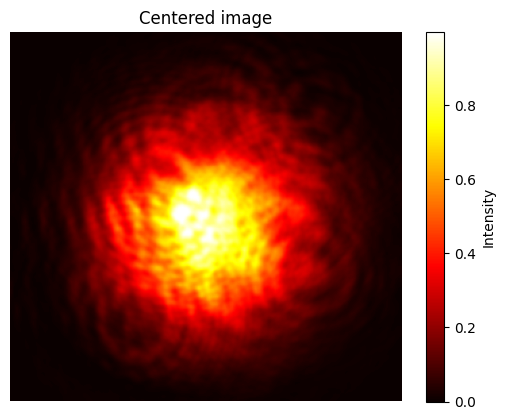
\includegraphics[width=1\linewidth]{Images/centered_example.png}
    \caption{2D representation of the beam on the camera.}
    \label{fig:centered_example}
\end{figure}

Figure~\ref{fig:centered_example} presents an example of the image files recorded for the experiment. As we can see, the image is centered in the position of the maximum amplitude and the beam has a circular profile, with a decreasing amplitude when leaving the center, as expected from a Gaussian beam. In Figure~\ref{fig:centered_example} we can see a 3D representation of the same beam, which shows the same characteristics: we can also notice that the surface has a lot of irregularities, which are due to external noise and dust on the surface of the camera. In order to remove these irregularities, one can use a Gaussian filter on the image, but the risk is to lose accuracy when studying the diffraction; thus, we proceed keeping this level of irregularities and using smooth Gaussian fits to compute the beam parameters.

\begin{figure}[!t]
    \centering
    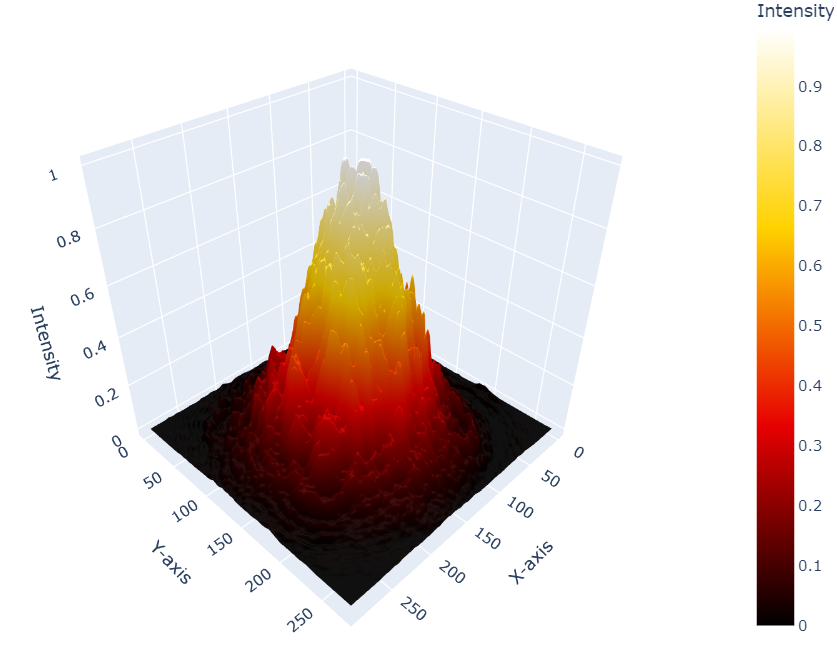
\includegraphics[width=1\linewidth]{Images/3d_example.png}
    \caption{3D representation of the beam on the camera.}
    \label{fig:3d_example}
\end{figure}

\begin{figure}[!h]
    \centering
    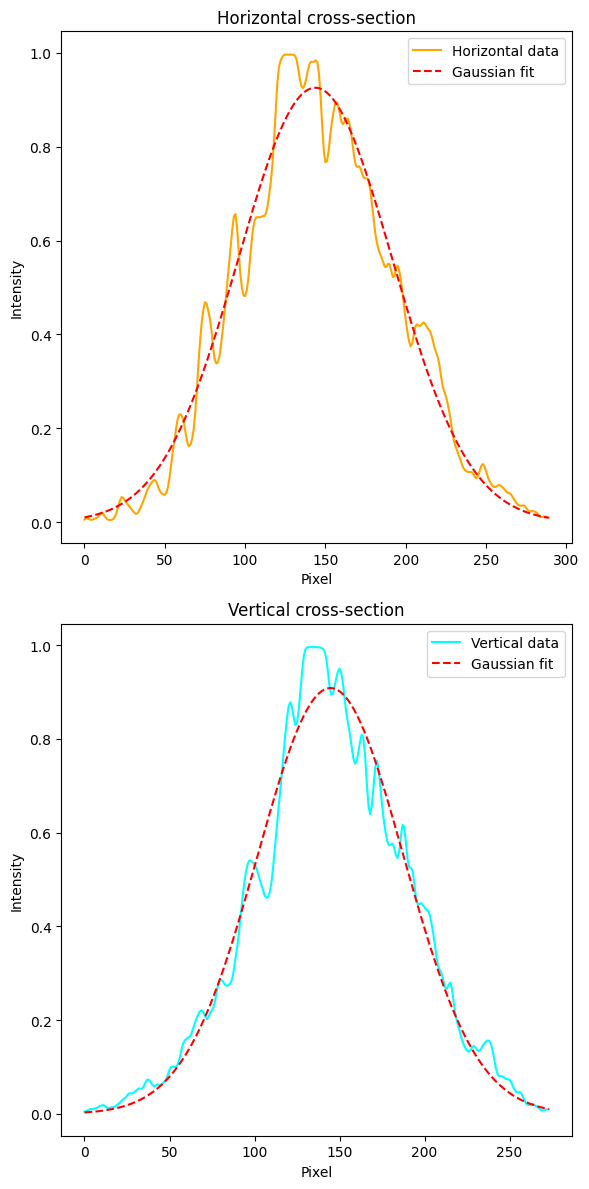
\includegraphics[width=0.87\linewidth]{Images/1d_gaussian_fit.png}
    \caption{1D Gaussian fit on the beam's profiles.}
    \label{fig:1d_gaussian_fit}
\end{figure}

We proceeded to fit the beam profile with a 2D Gaussian function, obtaining an ellipticity of \( 1.03 \pm 0.02 \). This result aligns with the expected value of \( 1 \), indicating that the beam should ideally exhibit a circular cross-section. The observed deviation is within acceptable experimental uncertainties. For clarity and to avoid overcrowding the paper with repetitive visualizations, we have not explicitly included the 2D Gaussian fit in the report. 

Instead, Figure~\ref{fig:1d_gaussian_fit} presents the 1D cross-section of the beam in correspondence with its maximum intensity. As shown, the profiles exhibit minor irregularities; however, the fits are of high quality in both axes. These fits allow us to extract key parameters of the Gaussian beam for all the recorded images during the experiment. The primary quantities of interest are the standard deviations along the two axes, as these determine the beam radius, as described in Section~\ref{sec:gaussian_beam_width}. The 2D beam radius is computed as the average of the two standard deviations obtained along the axes. Repeating this process for all available images provides a comprehensive characterization of the beam evolution when varying the distance $z$, which is presented in Figure~\ref{fig:beam_radius_fit}. Here, we plot the different beam radii varying the position and fit with Equation~\eqref{eq:beam_radius}: this procedure yields the following results for the two parameters, $W_0 = (2.96 \pm 0.12)\times 10^{-2} \; \text{cm}$ and $z_R = (45.99 \pm 2.14) \; \text{cm}$, which are in line with what expected. Moreover, these results are also in agreement with the relation between $W_0$ and $z_R$, expressed in~\eqref{eq:W_0_and_z_R}; for $\lambda=633 \;\text{nm}$, fixing $z_R$, we get   $W_0 = (3.04 \pm 0.28)\times 10^{-2} \; \text{cm}$, in agreement with the previous value.

\begin{figure}
    \centering
    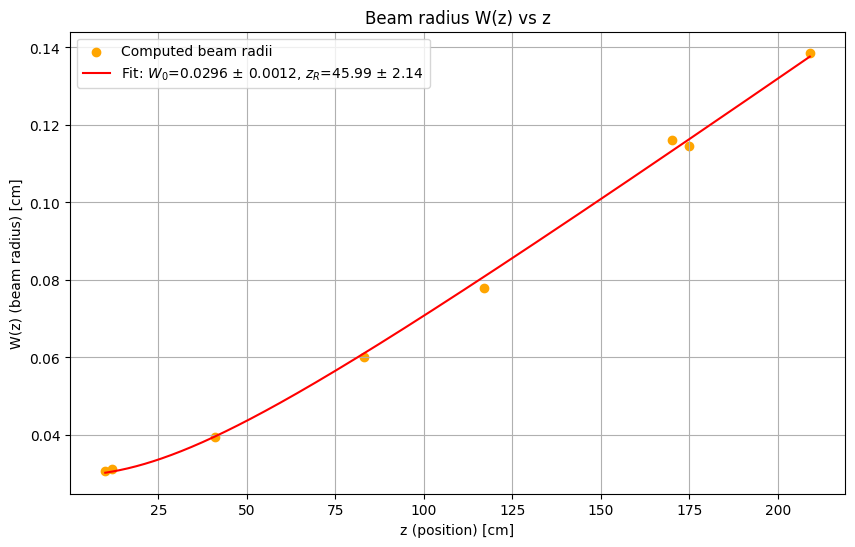
\includegraphics[width=\linewidth]{Images/beam_radius_fit.png}
    \caption{Beam radius at different distances.}
    \label{fig:beam_radius_fit}
\end{figure}

\begin{figure}[!b]
    \centering
    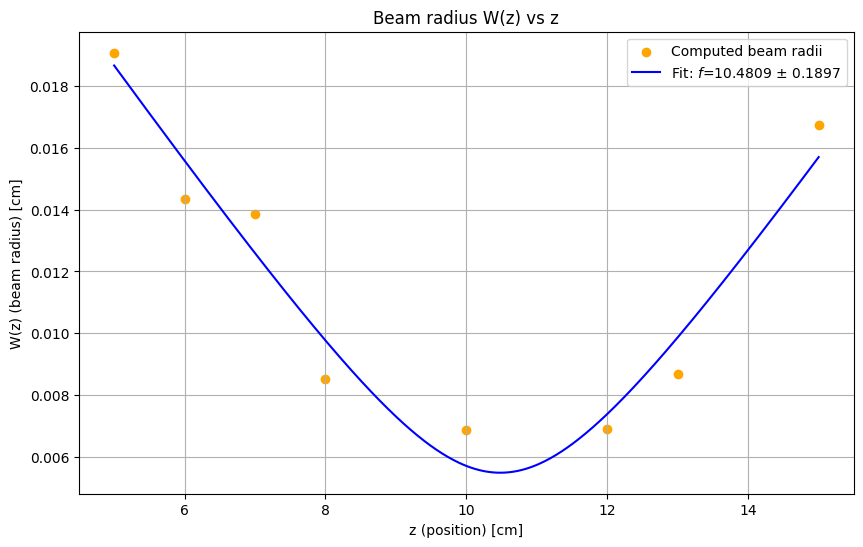
\includegraphics[width=\linewidth]{Images/beam_radius_lens_fit.png}
    \caption{Beam radius at different distances, with lens.}
    \label{fig:beam_radius_lens_fit}
\end{figure}

After this first phase, we proceeded to study how the lens modifies the behavior of the Gaussian beam. Assuming that the beam is collimated, meaning that its waist is positioned far enough from the lens, we observe that the beam retains the same Gaussian characteristics, but its dependency on $z$ changes due to the focal length of the lens. Consequently, the same analysis as in the previous phase was conducted, focusing on the beam radius as a function of the distance from the lens.
Figure~\ref{fig:beam_radius_lens_fit} presents the data and the corresponding fit, performed using Equation~\eqref{eq:beam_radius_lens}. As shown, the fit is of high quality, and the effect of the lens on the beam radius is clearly visible.; specifically, the fit yields a focal length of $f = (10.48 \pm 0.19) \, \text{cm}$ for the lens used in the experiment. This value corresponds to the minimum of the beam radius, which occurs when the distance $z$ is equal to $f$; beyond this point, both before and after $z = f$, the beam radius increases due to the focusing and divergence introduced by the lens. This behavior highlights the primary difference compared to the initial case of a freely propagating beam: while the beam radius evolves smoothly in the absence of a lens, the presence of a lens introduces a distinct minimum at $z = f$ and shows an enlargement of the beam for values of $z$ different than $f$.

\begin{figure}[!b]
    \centering
    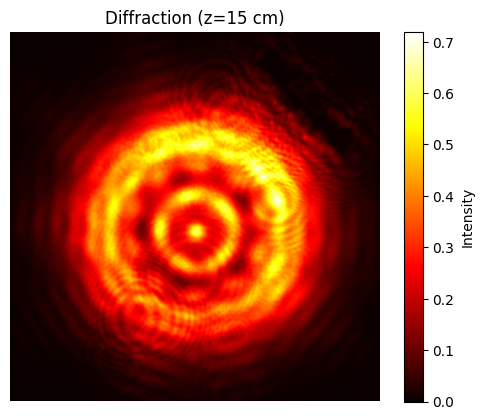
\includegraphics[width=\linewidth]{Images/diffraction_example.png}
    \caption{2D representation of the diffraction picture.}
    \label{fig:diffraction_example}
\end{figure}

\begin{figure}[!b]
    \centering
    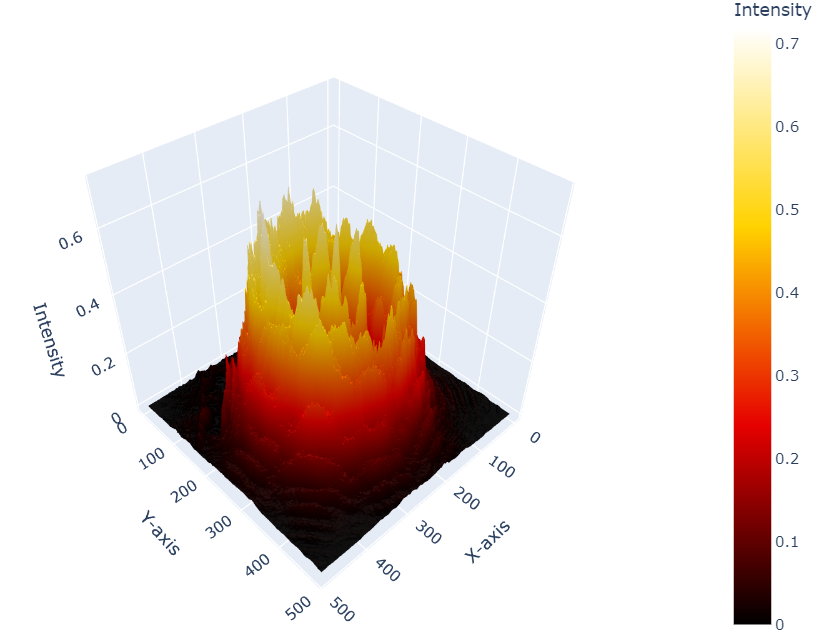
\includegraphics[width=\linewidth]{Images/3d_diffraction_example.png}
    \caption{3D representation of the diffraction picture.}
    \label{fig:3d_diffraction_example}
\end{figure}


Finally, the last part of the experiment focuses on diffraction. First, we examine the appearance of a diffracted beam. Figure~\ref{fig:diffraction_example} and Figure~\ref{fig:3d_diffraction_example} display the 2D and 3D representations of the diffraction pattern, respectively, for $z = 15 \, \text{cm}$. It is evident that we are observing a circular diffraction pattern characterized by alternating bright and dark concentric rings: this pattern is consistent with the expected outcome for a beam encountering an aperture, where the wavefronts interfere constructively and destructively. To analyze the diffraction quantitatively, we could have focused on the intensity profile of the pattern along a radial cross-section, comparing it with the theoretical prediction: due to lack of time and noise of the signal, we didn't do this analysis. We analyzed instead the Fresnel number $N_F$, defined in Equation~\eqref{eq:fresnel_number},in order to find the dimension of the slit. We can observe in~\ref{fig:diffraction_fit} the data (counted by observing the visible dark fringes in each image) and the corresponding fit; this has revealed a value of $a = 0.088 \pm 0.002 \, \text{cm}$, which is compatible with the expected result. We can also notice that, as the distance $z$ increases, the diffraction pattern evolves, transitioning gradually toward the far-field regime where the intensity profile becomes smoother and assumes a Gaussian distribution. This transition, which reflects the spreading of the beam and the dominance of far-field effects, is consistent with the theoretical predictions described in Section~\ref{sec:diffraction_theory}. 

\begin{figure}[!t]
    \centering
    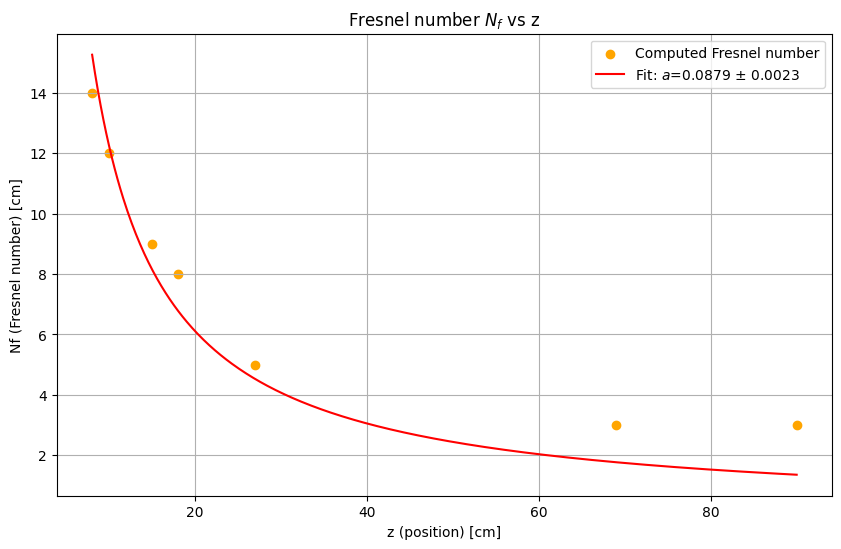
\includegraphics[width=\linewidth]{Images/diffraction_fit.png}
    \caption{Fresnel number for different distances.}
    \label{fig:diffraction_fit}
\end{figure}


\section{Conclusion}

In this experiment, we investigated the behavior of a Gaussian beam in various scenarios: free propagation, interaction with a lens and diffraction through a slit.

The free propagation analysis allowed us to determine the beam waist and Rayleigh; the obtained values of \( W_0 = (2.96 \pm 0.12) \times 10^{-2} \, \text{cm} \) and \( z_R = (45.99 \pm 2.14) \, \text{cm} \) align well with theoretical predictions, demonstrating the validity of the Gaussian beam approximation in our experimental setup. Additionally, the ellipticity confirms that the beam's cross-section is nearly circular.

Introducing a lens into the system provided further insights into the beam's behavior: the fitted focal length of agrees with the measured minimum beam radius at \( z = f \). Moreover, this analysis highlights how a lens focuses and subsequently diverges a Gaussian beam.

Finally, the diffraction study revealed a circular diffraction pattern, consistent with the interference effects expected, and we determined an aperture size in excellent agreement with the expected value. Moreover, as the distance \( z \) increased, the diffraction pattern transitioned from the near-field to the far-field regime, in agreement with theoretical predictions, providing further validation of our analysis.

In conclusion, this experiment demonstrates the theoretical and practical principles governing Gaussian beams: the strong agreement between experimental results and theoretical models underscores the robustness of the methods employed.




\section{Appendix}
\subsection{Experimental considerations}
\label{sec:appendix_exp_cons}
Obtaining a clean signal which can be used for correct data analysis is difficult, so we need to correctly address some issues:
\begin{itemize}
  \item \textbf{Background noise:}  
  It is essential to subtract a constant value representing the background noise from the transverse intensity distribution to obtain accurate plots.

  \item \textbf{CCD saturation:}  
  At certain distances, the laser beam intensity may saturate the CCD camera, causing the transverse intensity distributions to be clipped at the peak. Thus, proper attenuators are used to reduce the beam intensity, allowing the full plot to be displayed (care must be taken also to avoid damage to the camera from excessive beam intensity).

  \item \textbf{Dust:}  
  The presence of dust on the CCD camera can result in erroneous data collection: optical paper and a blower should be used to clean the camera surface thoroughly and measurements should be taken in areas of the camera with minimal dust contamination.
\end{itemize}

\section{Code}
All the data and the code for the data analysis can be found in this public Github repository: \href{https://github.com/Kallo27/QOL/tree/main/Lab3}{https://github.com/Kallo27/QOL/tree/main/Lab3}

\begin{thebibliography}{99}

\bibitem{pap1}
  A. E. Siegman, \textit{Lasers}, University Science Books (1986).

\bibitem{pap2}
  M. Born and E. Wolf, \textit{Principles of Optics}, 7th Edition, Cambridge University Press (1999).

\end{thebibliography}

\end{document}
